% ============================================================================
% CHAPTER 1H: BIOMEDICAL SYSTEMS
% ============================================================================

\section{Biomedical Systems}
\label{sec:biomedical}

Biomedical control systems interface with the human body, requiring special consideration for safety, variability between patients, and the inherent complexity of biological processes.

% ============================================================================
\subsection{Pharmacokinetics: Drug Distribution}
\label{subsec:pharmacokinetics}
% ============================================================================

Pharmacokinetics describes how drugs move through the body.

\subsubsection{One-Compartment Model}

\begin{figure}[htbp]
\centering
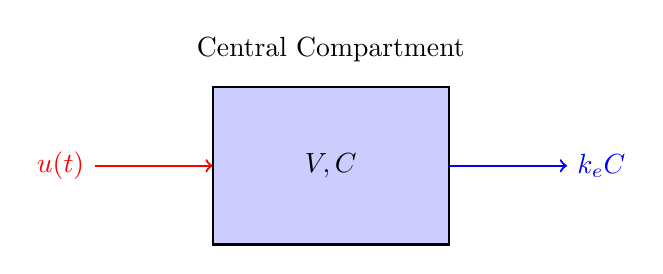
\begin{tikzpicture}
    % Compartment
    \draw[thick, fill=blue!20] (0,0) rectangle (3,2);
    \node at (1.5,1) {$V, C$};

    % Input (infusion)
    \draw[->, thick, red] (-1.5,1) -- (0,1) node[left, pos=0] {$u(t)$};

    % Elimination
    \draw[->, thick, blue] (3,1) -- (4.5,1) node[right] {$k_e C$};

    % Labels
    \node[above] at (1.5,2.2) {Central Compartment};
\end{tikzpicture}
\caption{One-compartment pharmacokinetic model.}
\label{fig:one_compartment}
\end{figure}

Mass balance:
\begin{equation}
V\frac{\dd C}{\dd t} = u(t) - k_e V C
\end{equation}

where:
\begin{itemize}
    \item $V$ = volume of distribution (L)
    \item $C$ = drug concentration (mg/L)
    \item $u(t)$ = infusion rate (mg/min)
    \item $k_e$ = elimination rate constant (1/min)
\end{itemize}

Transfer function:
\begin{equation}
\frac{C(s)}{U(s)} = \frac{1/V}{s + k_e}
\end{equation}

Half-life: $t_{1/2} = \ln(2)/k_e$

\begin{examplebox}[title=Example 1.15: IV Drug Infusion]
A drug has $V = 50$ L and $k_e = 0.1$ min$^{-1}$. Find:
\begin{enumerate}[label=(\alph*)]
    \item The half-life
    \item The infusion rate needed for steady-state concentration of 10 mg/L
    \item Time to reach 90\% of steady-state
\end{enumerate}

\textbf{Solution:}

(a) Half-life: $t_{1/2} = \ln(2)/0.1 = 6.93$ min

(b) At steady-state: $u_{ss} = k_e V C_{ss} = 0.1 \times 50 \times 10 = 50$ mg/min

(c) Time constant: $\tau = 1/k_e = 10$ min

Time to 90\%: $t = -\tau\ln(0.1) = 10 \times 2.3 = 23$ min
\end{examplebox}

\subsubsection{Two-Compartment Model}

\begin{figure}[htbp]
\centering
\begin{tikzpicture}[scale=1.1]
    % Central compartment box
    \draw[thick, fill=UofSCGarnet!25] (0.5,0.5) rectangle (3.5,2.5);
    \node[font=\large] at (2,1.5) {Central};
    \node[font=\small] at (2,0.9) {$V_1, C_1$};

    % Peripheral compartment box
    \draw[thick, fill=UofSCAtlantic!25] (5.5,0.5) rectangle (8.5,2.5);
    \node[font=\large] at (7,1.5) {Peripheral};
    \node[font=\small] at (7,0.9) {$V_2, C_2$};

    % Input arrow
    \draw[->, thick, UofSCHorseshoe] (-1.5,1.5) -- (0.5,1.5) node[left, pos=0, font=\small] {$u(t)$};
    \node[below, font=\tiny] at (-1.5,1.1) {Infusion};

    % Elimination from central compartment (downward)
    \draw[->, thick, UofSCCongaree] (2,0.5) -- (2,-0.7) node[below, font=\small] {$k_{10}C_1$};
    \node[right, font=\tiny] at (2.3,-0.2) {Elimination};

    % Transfer from central to peripheral (forward)
    \draw[->, thick, UofSCAtlantic] (3.5,1.8) -- (5.5,1.8);
    \node[above, midway, font=\small] {$k_{12}$};

    % Transfer from peripheral to central (backward)
    \draw[->, thick, UofSCGarnet] (5.5,1.2) -- (3.5,1.2);
    \node[below, midway, font=\small] {$k_{21}$};

    % Rate constant definitions
    \node[right, font=\tiny] at (9.2,2.2) {$k_{10}$ = elimination rate};
    \node[right, font=\tiny] at (9.2,1.8) {$k_{12}$ = central $\to$ peripheral};
    \node[right, font=\tiny] at (9.2,1.4) {$k_{21}$ = peripheral $\to$ central};
\end{tikzpicture}
\caption{Two-compartment pharmacokinetic model diagram showing drug infusion, inter-compartment transfer, and elimination with rate constants labeled.}
\label{fig:two_compartment}
\end{figure}

Mass balances:
\begin{align}
V_1\frac{\dd C_1}{\dd t} &= u(t) - (k_{10} + k_{12})V_1 C_1 + k_{21}V_2 C_2 \\
V_2\frac{\dd C_2}{\dd t} &= k_{12}V_1 C_1 - k_{21}V_2 C_2
\end{align}

This yields a second-order system with two exponential phases:
\begin{itemize}
    \item \textbf{Distribution phase} ($\alpha$): rapid initial decline
    \item \textbf{Elimination phase} ($\beta$): slower terminal decline
\end{itemize}

% ============================================================================
\subsection{Glucose-Insulin Dynamics}
\label{subsec:glucose}
% ============================================================================

\begin{figure}[htbp]
\centering
\begin{tikzpicture}[node distance=2.8cm, x=1cm, y=1cm]
    % Glucose box
    \draw[thick, fill=UofSCGarnet!25] (-1,0.8) rectangle (1,1.8);
    \node[font=\large] at (0,1.3) {Glucose $G$};

    % Insulin box
    \draw[thick, fill=UofSCAtlantic!25] (-1,-1.2) rectangle (1,-0.2);
    \node[font=\large] at (0,-0.7) {Insulin $I$};

    % Meal input arrow
    \draw[->, thick, UofSCHorseshoe] (-2.8,1.3) -- (-1,1.3) node[left, pos=0, font=\small] {Meal $D$};

    % Insulin injection arrow
    \draw[->, thick, UofSCHorseshoe] (-2.8,-0.7) -- (-1,-0.7) node[left, pos=0, font=\small] {Injection $u$};

    % Glucose utilization arrow
    \draw[->, thick, UofSCCongaree] (1,1.3) -- (2.8,1.3) node[right, pos=1, font=\small] {Utilization};

    % Insulin clearance arrow
    \draw[->, thick, UofSCCongaree] (1,-0.7) -- (2.8,-0.7) node[right, pos=1, font=\small] {Clearance};

    % Insulin enhances glucose uptake (upward arrow from insulin to glucose)
    \draw[->, thick, UofSCAtlantic] (0.3,-0.2) -- (0.3,0.8) node[midway, right, font=\small] {Enhances};
    \node[right, font=\tiny] at (0.6,0.3) {uptake};

    % Glucose stimulates insulin secretion (downward arrow from glucose to insulin)
    \draw[->, thick, UofSCGarnet] (-0.3,0.8) -- (-0.3,-0.2) node[midway, left, font=\small] {Stimulates};
    \node[left, font=\tiny] at (-0.8,0.3) {secretion};
\end{tikzpicture}
\caption{Glucose-insulin feedback loop block diagram showing meal and infusion inputs, utilization/clearance outputs, and the bidirectional regulatory feedback.}
\label{fig:glucose_insulin}
\end{figure}

\subsubsection{Minimal Model (Bergman)}

\begin{align}
\frac{\dd G}{\dd t} &= -p_1 G - X(G + G_b) + D(t) \\
\frac{\dd X}{\dd t} &= -p_2 X + p_3(I - I_b) \\
\frac{\dd I}{\dd t} &= -n(I - I_b) + \gamma(G - h)^+ + u(t)
\end{align}

where:
\begin{itemize}
    \item $G$ = glucose concentration (mg/dL)
    \item $I$ = insulin concentration ($\mu$U/mL)
    \item $X$ = insulin action (remote compartment)
    \item $D(t)$ = meal disturbance
    \item $u(t)$ = insulin infusion (for artificial pancreas)
\end{itemize}

\subsubsection{Linearized Model for Control Design}

Near operating point $(G_0, I_0)$:
\begin{equation}
\begin{bmatrix} \Delta\dot{G} \\ \Delta\dot{I} \end{bmatrix} =
\begin{bmatrix} -p_1 - X_0 & -K_G \\ K_I & -n \end{bmatrix}
\begin{bmatrix} \Delta G \\ \Delta I \end{bmatrix} +
\begin{bmatrix} 1 \\ 0 \end{bmatrix} \Delta D +
\begin{bmatrix} 0 \\ 1 \end{bmatrix} \Delta u
\end{equation}

% ============================================================================
\subsection{Cardiovascular System}
\label{subsec:cardiovascular}
% ============================================================================

\subsubsection{Windkessel Model}

The arterial system can be modeled as an electrical analog:

\begin{figure}[htbp]
\centering
\begin{circuitikz}[scale=1]
    % Current source (heart)
    \draw (0,0) to[I, l=$Q(t)$] (0,2);

    % Capacitor (arterial compliance)
    \draw (0,2) -- (2,2) to[C, l=$C$] (2,0) -- (0,0);

    % Resistor (peripheral resistance)
    \draw (2,2) -- (4,2) to[R, l=$R$] (4,0) -- (2,0);

    % Pressure labels
    \node[above] at (1,2.2) {$P(t)$};
\end{circuitikz}
\caption{Two-element Windkessel model.}
\label{fig:windkessel}
\end{figure}

Governing equation:
\begin{equation}
C\frac{\dd P}{\dd t} + \frac{P}{R} = Q(t)
\end{equation}

where:
\begin{itemize}
    \item $P$ = arterial pressure (mmHg)
    \item $Q$ = cardiac output (mL/s)
    \item $C$ = arterial compliance (mL/mmHg)
    \item $R$ = systemic vascular resistance (mmHg$\cdot$s/mL)
\end{itemize}

\subsubsection{Blood Pressure Control}

The baroreflex regulates blood pressure:
\begin{equation}
\frac{\dd P}{\dd t} = -\frac{1}{\tau_P}(P - P_{\text{set}}) + K_u u(t)
\end{equation}

where $u(t)$ represents vasoactive drug infusion.

% ============================================================================
\subsection{Respiratory System}
\label{subsec:respiratory}
% ============================================================================

\subsubsection{Mechanical Ventilation Model}

\begin{figure}[htbp]
\centering
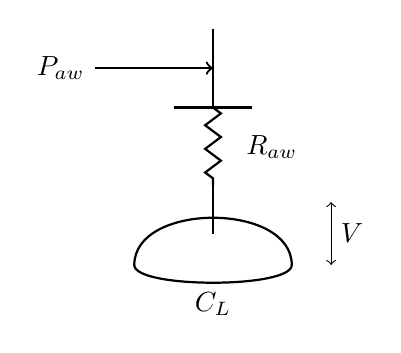
\begin{tikzpicture}
    % Airways
    \draw[thick] (0,3) -- (0,2);
    \draw[thick] (-0.5,2) -- (0.5,2);

    % Resistance
    \draw[thick, decorate, decoration={zigzag, segment length=3mm, amplitude=1mm}]
        (0,2) -- (0,1);
    \node[right] at (0.3,1.5) {$R_{aw}$};

    % Lung (compliance)
    \draw[thick] (-1,0) .. controls (-1,0.8) and (1,0.8) .. (1,0);
    \draw[thick] (-1,0) .. controls (-1,-0.3) and (1,-0.3) .. (1,0);
    \node at (0,-0.5) {$C_L$};

    % Connection
    \draw[thick] (0,1) -- (0,0.4);

    % Pressure labels
    \draw[->, thick] (-1.5,2.5) -- (0,2.5) node[left, pos=0] {$P_{aw}$};
    \draw[<->] (1.5,0) -- (1.5,0.8) node[right, midway] {$V$};
\end{tikzpicture}
\caption{Single-compartment lung model.}
\label{fig:lung_model}
\end{figure}

Equation of motion:
\begin{equation}
P_{aw} = R_{aw}\dot{V} + \frac{V}{C_L} + P_{\text{PEEP}}
\end{equation}

where:
\begin{itemize}
    \item $P_{aw}$ = airway pressure (cmH$_2$O)
    \item $R_{aw}$ = airway resistance (cmH$_2$O$\cdot$s/L)
    \item $C_L$ = lung compliance (L/cmH$_2$O)
    \item $V$ = lung volume (L)
    \item $P_{\text{PEEP}}$ = positive end-expiratory pressure
\end{itemize}

Transfer function:
\begin{equation}
\frac{V(s)}{P_{aw}(s)} = \frac{C_L}{R_{aw}C_L s + 1}
\end{equation}

% ============================================================================
\subsection{Anesthesia Delivery}
\label{subsec:anesthesia}
% ============================================================================

\subsubsection{Propofol Pharmacokinetics}

Three-compartment mammillary model:
\begin{align}
V_1\dot{C}_1 &= u - k_{10}V_1 C_1 - k_{12}V_1 C_1 + k_{21}V_2 C_2 - k_{13}V_1 C_1 + k_{31}V_3 C_3 \\
V_2\dot{C}_2 &= k_{12}V_1 C_1 - k_{21}V_2 C_2 \\
V_3\dot{C}_3 &= k_{13}V_1 C_1 - k_{31}V_3 C_3
\end{align}

\subsubsection{Pharmacodynamic Effect}

The effect-site concentration $C_e$ relates to the measured output (e.g., BIS index):
\begin{equation}
\frac{\dd C_e}{\dd t} = k_{e0}(C_1 - C_e)
\end{equation}

Hill equation for effect:
\begin{equation}
\text{Effect} = E_0 - E_{\max}\frac{C_e^\gamma}{C_e^\gamma + EC_{50}^\gamma}
\end{equation}

% ============================================================================
\subsection{Medical Device Examples}
\label{subsec:medical_devices}
% ============================================================================

\subsubsection{Infusion Pump}

Transfer function (actuator dynamics):
\begin{equation}
\frac{Q(s)}{V_{\text{cmd}}(s)} = \frac{K_p}{\tau_p s + 1}
\end{equation}

where $Q$ is flow rate and $V_{\text{cmd}}$ is the command voltage.

\subsubsection{Pacemaker Rate Response}

Activity-based pacing rate:
\begin{equation}
\tau\frac{\dd R}{\dd t} + R = R_{\text{base}} + K \cdot A(t)
\end{equation}

where $A(t)$ is the activity sensor signal and $R$ is the pacing rate.

\subsubsection{Cochlear Implant Signal Processing}

Filter bank model:
\begin{equation}
H_k(s) = \frac{\omega_k^2}{s^2 + 2\zeta\omega_k s + \omega_k^2}
\end{equation}

for frequency band $k$ centered at $\omega_k$.

% ============================================================================
\subsection{Neural Systems}
\label{subsec:neural}
% ============================================================================

\subsubsection{Hodgkin-Huxley Neuron Model}

\begin{equation}
C_m\frac{\dd V}{\dd t} = I_{\text{ext}} - g_{Na}m^3h(V - E_{Na}) - g_K n^4(V - E_K) - g_L(V - E_L)
\end{equation}

with gating variables $m$, $h$, $n$ following first-order kinetics.

\subsubsection{Simplified Integrate-and-Fire Model}

\begin{equation}
\tau_m\frac{\dd V}{\dd t} = -(V - V_{\text{rest}}) + R_m I_{\text{ext}}
\end{equation}

When $V$ reaches threshold $V_{th}$, the neuron fires and resets.

% ============================================================================
\subsection{Exercises: Biomedical Systems}
% ============================================================================

\begin{exercise}
A drug has one-compartment kinetics with $V = 35$ L and $t_{1/2} = 4$ hours.
\begin{enumerate}[label=(\alph*)]
    \item Calculate the elimination rate constant
    \item Find the loading dose to achieve 20 mg/L immediately
    \item Find the maintenance infusion rate
    \item Write the transfer function from infusion rate to concentration
\end{enumerate}
\end{exercise}

\begin{exercise}
A patient's arterial compliance is $C = 2$ mL/mmHg and peripheral resistance is $R = 1$ mmHg$\cdot$s/mL.
\begin{enumerate}[label=(\alph*)]
    \item Find the time constant of the arterial system
    \item If cardiac output steps from 80 to 100 mL/s, find the new steady-state pressure
    \item Sketch the pressure response to the step change
\end{enumerate}
\end{exercise}

\begin{exercise}
A mechanical ventilator delivers pressure to a patient with $R_{aw} = 10$ cmH$_2$O$\cdot$s/L and $C_L = 0.05$ L/cmH$_2$O.
\begin{enumerate}[label=(\alph*)]
    \item Find the time constant
    \item If inspiratory pressure is 20 cmH$_2$O above PEEP, find the tidal volume
    \item Find the inspiratory time needed to achieve 95\% of the tidal volume
\end{enumerate}
\end{exercise}

\begin{exercise}
An artificial pancreas controller must regulate glucose. The simplified model has:
\begin{equation}
\frac{G(s)}{U(s)} = \frac{-2}{(10s+1)(50s+1)}
\end{equation}
where $G$ is glucose (mg/dL) and $U$ is insulin (U/hr), with time in minutes.
\begin{enumerate}[label=(\alph*)]
    \item Find the steady-state glucose change for 1 U/hr insulin increase
    \item Find the system poles and time constants
    \item Sketch the glucose response to a step insulin input
\end{enumerate}
\end{exercise}

\begin{exercise}
A two-compartment drug delivery system has: $V_1 = 10$ L, $V_2 = 40$ L, $k_{10} = 0.2$ hr$^{-1}$, $k_{12} = 0.15$ hr$^{-1}$, and $k_{21} = 0.1$ hr$^{-1}$.
\begin{enumerate}[label=(\alph*)]
    \item Calculate the drug concentration in both compartments at 4 hours following a 500 mg IV bolus dose
    \item Find the half-lives for the distribution and elimination phases
    \item If the drug is continuously infused at 10 mg/hr, find the steady-state concentrations in both compartments
\end{enumerate}
\end{exercise}

\begin{exercise}
A patient receiving mechanical ventilation has measured respiratory mechanics: $R_{aw} = 8$ cmH$_2$O$\cdot$s/L, $C_L = 0.04$ L/cmH$_2$O, $I_r = 0.03$ L/cmH$_2$O (chest wall compliance).
\begin{enumerate}[label=(\alph*)]
    \item Find the total respiratory system compliance and time constant
    \item For a constant inspiratory pressure of 15 cmH$_2$O (above PEEP), calculate tidal volume after 5 time constants
    \item Design a pressure control strategy to deliver 0.5 L tidal volume in 1 second
\end{enumerate}
\end{exercise}

\begin{exercise}
A pacemaker rate-response control system regulates heart rate based on activity. The transfer function from activity sensor voltage to pacing rate is:
\begin{equation}
\frac{R(s)}{A(s)} = \frac{K}{0.5s + 1}, \quad K = 100 \text{ bpm/V}
\end{equation}
\begin{enumerate}[label=(\alph*)]
    \item Calculate the steady-state pacing rate for activity input of 0.5 V
    \item Find the time to reach 90\% of steady-state rate
    \item Design a controller to achieve 0 to 120 bpm range with sensor output of 0 to 1 V
\end{enumerate}
\end{exercise}

\begin{exercise}
An infusion pump delivers IV medications with first-order actuator dynamics: $\frac{Q(s)}{V_{\text{cmd}}(s)} = \frac{K_p}{\tau_p s + 1}$, where $K_p = 5$ mL/min/V and $\tau_p = 0.1$ s.
\begin{enumerate}[label=(\alph*)]
    \item For a step command of 2 V, find the steady-state flow rate
    \item Calculate the actual flow rate at time $t = 0.2$ s
    \item If a patient needs 50 mL of drug infused in exactly 10 minutes, determine the required command voltage accounting for actuator dynamics
\end{enumerate}
\end{exercise}

\begin{exercise}
A prosthetic limb controller uses proportional myoelectric control, with muscle EMG signal driving joint angle:
\begin{equation}
\theta(s) = \frac{G(s)}{1 + G(s)H(s)}E(s)
\end{equation}
where $G(s) = \frac{K}{\tau s + 1}$ (actuator), $H(s) = K_f s$ (feedback with damping), $K = 45$ deg/V, $\tau = 0.2$ s, and $K_f = 0.1$ V$\cdot$s/deg.
\begin{enumerate}[label=(\alph*)]
    \item Find the closed-loop transfer function $\theta(s)/E(s)$
    \item For a step EMG input of 0.5 V, calculate steady-state joint angle
    \item Sketch the response and identify if overshoot or oscillation occurs
    \item Design a proportional controller to add to $G(s)$ that achieves 1 deg/V steady-state sensitivity with damping ratio 0.8
\end{enumerate}
\end{exercise}

\begin{exercise}
A glucose-insulin model for artificial pancreas design is based on the Bergman minimal model. Patient parameters are: $p_1 = 0.03$ min$^{-1}$, $p_2 = 0.02$ min$^{-1}$, $p_3 = 1.2 \times 10^{-5}$ mL$/$($\mu$U$\cdot$min$)$, $n = 0.1$ min$^{-1}$, $\gamma = 0.5$ mg$/$dL$/min$/($\mu$U$/mL$)$, with $G_b = 95$ mg/dL and $I_b = 12$ $\mu$U/mL.
\begin{enumerate}[label=(\alph*)]
    \item Linearize the system about the basal operating point $(G_0, I_0) = (G_b, I_b)$
    \item Find the transfer functions $G(s)/U(s)$ and $G(s)/D(s)$
    \item Design a proportional insulin infusion controller: $u(t) = K_p(G_{\text{ref}} - G(t))$ that regulates glucose to 100 mg/dL with settling time under 3 hours
\end{enumerate}
\end{exercise}
